\documentclass[aps,prl, reprint]{revtex4-2}
%\usepackage[margin=0.5in]{geometry} 
\usepackage{graphicx}% Include figure files
\usepackage{dcolumn}% Align table columns on decimal point
%\usepackage{bm}% bold math
%\usepackage[mathlines]{lineno}% Enable numbering of text and display math
%\usepackage{hyperref}% add hypertext capabilities
%\usepackage{relsize}
%\usepackage[usenames,dvipsnames,svgnames,table]{xcolor}
%\usepackage{proofread}
%\newcommand{\bd}[1] {\frac{#1}{b}}
%\usepackage{comment}
%\usepackage{amsmath,amsthm,amssymb,scrextend}
\usepackage{physics, qcircuit}
\usepackage{breqn}
%\usepackage{url}
\usepackage{natbib, courier, breqn}
\bibliographystyle{apsrev4-2}


\begin{document}
\title{Simulating the Heisenberg Model}
\date{\today}
\author{Timothy Skaras}
\affiliation{Department of Physics$,$ Cornell University$,$ Ithaca$,$ New York$,$ 14853}
\begin{abstract}
We estimate the entanglement entropy of the GHZ state using both simulated and real measurement data. We use Qiskit to measure the target state in the Pauli basis and then use the classical shadows protocol to estimate the entanglement entropy from our measurement data. Our estimated value aligns very well with theory for our simulated data (relative error $\leq 0.15\%$), but our estimated value based on real data differs substantially from the theoretical value for our target state (relative error $\approx 20\%$). We conclude that the device's large error is most likely caused by noise.
\end{abstract}

\maketitle

\section{Introduction}

It is well known that quantum mechanical systems are difficult to solve with classical computers due to the exponential nature of quantum systems. The state space of a classical system grows linearly with the number of particles. For instance, if you are studying classical particles in a 3D box, you only need an additional 6 parameters to specify the state of the system with one more particle (3 positions and 3 momenta). In contrast, if you have spin-$\frac{1}{2}$ particles on a lattice, the size of the Hilbert space doubles with each particle you add, so in the worst case you need twice as much memory to specify the wave function of such a system. 

In 1982, Richard Feynman proposed a way of getting around this exponential scaling problem: use quantum mechanical systems to simulate quantum mechanical systems -- in other words, use a quantum computer \cite{feynman1982simulating}. For instance, if you are interested in computing dynamics, quantum computers are advantageous because the coefficient on each basis vector in the Hilbert space is not explicitly specified or stored, so quantum computers do not have this exponential problem. As the state space grows, computing dynamics becomes even more difficult because the number of elements in an unitary matrix is the square of the Hilbert space dimension. Quantum computing allows us to avoid these problems, which is why quantum computers hold immense potential for advancing our understanding of condensed matter systems.

Theoretically, time evolving a quantum state on a quantum computer with a given Hamiltonian is as simple as adding the right unitary gate to the quantum circuit. Most real quantum devices, however, have a finite gate set, and it is usually not possible to implement the time evolution operator exactly on the quantum computer. If the gate set is universal, it is guaranteed that we can implement a gate that is arbitrarily close to the correct time evolution operator (assuming perfect fidelity). Quantum simulation is the task of finding ways to approximate and implement time evolution operators with a limited gate set \cite{lloyd1996universal}.

In this paper, we will use quantum simulation techniques to simulate the dynamics of the Heisenberg model. The Heisenberg model is a quantum mechanical model that describes the magnetic interactions of spins on a lattice. We will be working with three spin-$\frac{1}{2}$ particles in 1D, and our goal will be to use Qiskit to simulate the dynamics with as high a fidelity as possible on the \texttt{ibmq\_jakarta} device, a 7 qubit quantum computer hosted by IBM.
\begin{figure}[b]
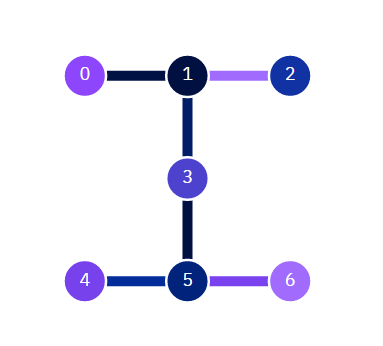
\includegraphics[width=0.4\textwidth]{JakartaDiagram.png}
\caption{This figure depicts how the qubits of the \texttt{ibmq\_jakarta} device are connected to one another. Two qubit gates can only be performed on connected qubits.}
\label{fig:JakartaConnect}
\end{figure}
\section{Experimental Hardware}

For our simulation task we will be using the \texttt{ibmq\_jakarta} device. This is a 7 qubit quantum computer whose qubits are connected as depicted in figure \ref{fig:JakartaConnect}. Our simulation task will require us to use gates on this device, but like many other devices \texttt{ibmq\_jakarta} has a limited gate set. This means that any gate we want to execute on the device must either be in the gate set or must be broken down into some composition of gates in the gate set. The gate set on this device consists of $R_z(\theta)$, $X$, $\sqrt{X}$, and $CNOT$ gates. The first gate $R_z(\theta)$ is an arbitrary single qubit rotation about the z-axis. The second is the $\sigma^{x}$ or NOT gate. The third $\sqrt{X}$ is the square root of the NOT gate, and the last $CNOT$ is the controlled not gate. We note that $\sqrt{X}$ is equivalent (differs only by a global phase) to a $\pi/2$ rotation about the x-axis $R_x(\pi/2)$.

\section{Quantum Simulation}

The Heisenberg model, in its most general form, is defined as
\begin{dmath}
H =- \sum_{j=1}^{N}\left(J_{x} \sigma_{j}^{x} \sigma_{j+1}^{x}+J_{y} \sigma_{j}^{y} \sigma_{j+1}^{y}\\
+J_{z} \sigma_{j}^{z} \sigma_{j+1}^{z}+h \sigma_{j}^{z}\right),
\end{dmath}
where $h$ is the external magnetic field and $J_x$, $J_y$, and $J_z$ are the couplings along the x, y, and z directions respectively. The subscript $j$ denotes the site that each spin operator is acting on, and $\sigma$'s are the pauli matrices which are given by 
\begin{equation}
\begin{array}{c}
\sigma^{x}=\left(\begin{array}{cc}
0 & 1 \\
1 & 0
\end{array}\right), \,
\sigma^{y}=\left(\begin{array}{cc}
0 & -i \\
i & 0
\end{array}\right),\,
\sigma^{z}=\left(\begin{array}{cc}
1 & 0 \\
0 & -1
\end{array}\right)
\end{array}
\end{equation}
when written in the z-basis. We will be considering the XXX Heisenberg model where $J = J_x = J_y = J_z$ and $h =0$. For simplicity, we will assume $J=1$ throughout this paper.  

The Heisenberg model is useful for studying the studying the dynamics and behavior of quantum mechanical magnetic interactions of spins. We will be simulating the quantum mechanical version of the Heisenberg model on three spin-$\frac{1}{2}$ particles. For our task, we start with the initial condition
\begin{equation}
\ket{\psi(t=0)} = \ket{110}
\end{equation}
with open boundary conditions and seek to simulate a total amount of time $\tau = \pi$. Theoretically, the time evolution of this initial condition is determined by the time-evolution operator
\begin{equation}
\ket{\psi(t=\tau)} = e^{-i \hat{H} \tau}\ket{\psi(0)},
\end{equation}
where we have set $\hbar = 1$. For our problem the time evolution operator is the exponential of a sum of pauli strings. For instance, we could generically write the hamiltonian as
\begin{equation}
H = \sum_i h_i
\end{equation}
where each of the $h_i$'s is the tensor product of two pauli matrices on two nearest neighbor sites. It is fairly straightforward to implement the unitary evolution of each $h_i$ taken individually. For instance, suppose we wanted to implement
\begin{equation}
e^{-i \sigma^{z}_1 \otimes \sigma^{z}_2 t}.
\label{eqn:rzz}
\end{equation}
Our native gate set lets us do single-qubit z-rotations which are defined as
\begin{equation}
R_{z}(2t)=e^{-i \sigma^{z}_1 \otimes I t },
\end{equation}
where the identity is made explicit for clarity. We can turn this into a two qubit rotation by noticing that a $Z$ gate with a CNOT on either side is equivalent to a Z gate on two qubits, i.e., CNOT $(\sigma^{z} \otimes I)$ CNOT = $\sigma^{z} \otimes \sigma^{z}$. This relationship still holds when $\sigma^{z} \otimes I$ is in an exponential (see figure \ref{fig:rzz}). 
\begin{figure}[t]
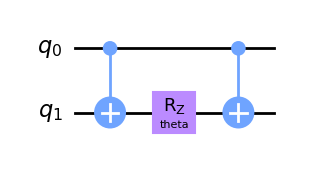
\includegraphics[width=0.35\textwidth]{Rzz.png}
\caption{This circuit shows a z-rotation sandwiched between two CNOT gates. This circuit is equivalent to the two qubit rotation given in equation (\ref{eqn:rzz}).}
\label{fig:rzz}
\end{figure}
Additionally, by using the Hadamard gate $H$ and the phase gate $S$ we can exploit relationships such as $HZH = X$ and $S X S^{\dagger}=Y$ to build other unitaries generated by individual $h_i$. This is not sufficient, however. The different $h_i$ do not commute, so we cannot split the exponential of the sum into the product of exponentials. It is for this reason that we must use a technique known as trotterization.

Generally speaking, if we have two matrices $h_1$ and $h_2$
\begin{equation}
e^{(h_1 + h_2)t} \neq e^{h_1 t}e^{h_2 t}.
\end{equation}
Though the two sides of this equation are not equal, they are approximately true when $t$ is small. If we want to simulate to a time $t$, we need only split the total time into $N$ steps and apply the two gates successively. More precisely
\begin{align}
e^{(h_1 + h_2)t}&=\lim _{n \rightarrow \infty}\left(e^{h_1 t/ n} e^{h_2 t / n}\right)^{n}\\
&\approx \left(e^{h_1 t / N} e^{h_2 t/ N}\right)^{N}.
\end{align}
Using the Zassenhaus formula 
\begin{align*}
e^{t(h_1+h_2)}&=e^{t h_1} e^{t h_2} e^{-\frac{t^{2}}{2}[h_1, h_2]}\cdots\\
&= e^{t h_1} e^{t h_2}(1 -\frac{t^{2}}{2}[h_1, h_2] + \cdots)\\
&=e^{t h_1} e^{t h_2} + \mathcal{O}(t^2),
\end{align*}
we can see that this trotterization method has a second-order accuracy \cite{dupays2021closed}.
\begin{figure*}[t]
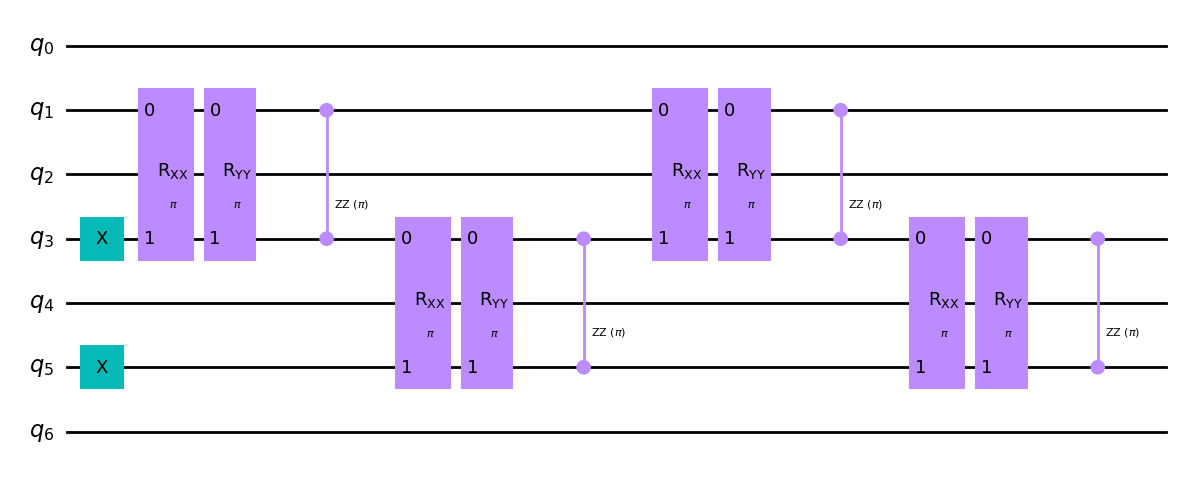
\includegraphics[width=\textwidth]{../Trotterization.png}
\caption{Circuit diagram of trotterization with two steps. The gates $R_{xx}$, $R_{yy}$, $R_{zz}$ are two qubit rotations (e.g., equation \ref{eqn:rzz} is $R_{zz}(2t)$). The qubits are all initially in the $\ket{0}$ state, and the two $X$ gates flip two qubits to give us the initial condition $\ket{110}$ on qubits 5, 3, and 1 respectively.}
\label{fig:TrotterCircuit}
\end{figure*}

Recalling the commutation relations for pauli matrices
\begin{equation}
[\sigma^{i}, \sigma^{j}] = 2i \epsilon_{ijk}\sigma^{k}, \quad \{\sigma^{i}, \sigma^{j}\} = 2\delta_{ij	},
\end{equation}
where $i,j,k$ can be $1,2,$ or 3 for each possible axis, we see that different pauli matrices do not commute and will actually anticommute. So for instance, the term $\sigma_{1}^{x} \sigma_{2}^{x}$ will commute with other terms acting on the same two sites such as $\sigma_{1}^{y} \sigma_{2}^{y}$ but will not commute with terms such as $\sigma_{2}^{z} \sigma_{3}^{z}$.

Because our system is only three qubits, we can easily write out the full time evolution operator
\begin{dmath}
U(t) = \exp\left[-i(\sigma_{1}^{x} \sigma_{2}^{x} + \sigma_{1}^{y} \sigma_{2}^{y} + \sigma_{1}^{z} \sigma_{2}^{z} \\
+ \sigma_{2}^{x} \sigma_{3}^{x} + \sigma_{2}^{y} \sigma_{3}^{y} + \sigma_{2}^{z} \sigma_{3}^{z})t\right].
\end{dmath}
With trotterization over N time steps this becomes
\begin{align*}
U(t) &\approx \left(e^{\frac{-it}{N}\sum_\gamma\sigma_{1}^{\gamma} \sigma_{2}^{\gamma}}e^{\frac{-it}{N}\sum_\gamma\sigma_{2}^{\gamma} \sigma_{3}^{\gamma}}\right)^N\\
&\approx \left(\prod_{\gamma}e^{\frac{-it}{N}\sigma_{1}^{\gamma} \sigma_{2}^{\gamma}}\prod_{\gamma}e^{\frac{-it}{N}\sigma_{2}^{\gamma} \sigma_{3}^{\gamma}}\right)^N,
\end{align*}
where the sums/products are over $\gamma =x,y,z$. No additional approximation has been made between the first and second lines because the pauli strings acting on the same sites commute. We have now simplified the time evolution operator into unitary gates that we can directly implement on the quantum device. In figure \ref{fig:TrotterCircuit} we show an example of a trotterized circuit with $N=2$. Note that this circuit has not been compiled for our specific device, so when the circuit is executed the two qubit gates will need to be decomposed into gates that are in our gate set.

\section{Simulation Results}

It is difficult to obtain access to the \texttt{ibmq\_jakarta} device, so we will first optimize our circuit using noise models on simulators. Our goal is to simulate the Heisenberg model for a total time $\tau=\pi$ with the highest fidelity possible. This amount of time $\tau$ is convenient because our specific initial condition $\ket{\psi(0)}=\ket{110}$ returns exactly to its initial state $\ket{\psi(\tau)}=\ket{110}$ after this length of time. Before we can compute the quantum fidelity of the final state on our circuit, we must first determine what the state is. On a real device, we do not have direct access to the exact state and must reconstruct the state based on measurement outcomes. So, we perform measurements in the pauli basis and use built-in Qiskit routines to do quantum tomography [citation].

Let $\tilde{\rho}$ be the state reconstruction output from our quantum tomography process and let $\rho = \dyad{110}$ be our target state. Because our target state is pure, the quantum fidelity has a simple formula
\begin{equation}
F(\rho, \tilde{\rho}) = \Tr[\rho\tilde{\rho}].
\end{equation}
Theoretically on a perfect device, more trotter steps improves the accuracy of the time-evolution operator and hence increases the fidelity of the final state. In practice, however, the devices are very noisy and adding trotter steps will eventually make the fidelity worse. Using noise models on simulators will allow us to quickly determine the optimal number of trotter steps. 

In figure \ref{fig:SimFids}, we show how adding more trotter steps (increasing N) changes the fidelity of the final state. We see that in the absence of noise (orange line) the fidelity monotonically increases with the number of trotter steps as expected. Once we account for noise, however, we see the fidelity actually gets worse after 9 trotter steps (blue line). The error bars indicate the standard deviation of the computed fidelity over 15 repetitions. Each repetition consists of 8192 shots on each tomography circuit (8192 measurements in each basis).

The noise models take into account characteristics specific to the device we are trying to simulate \texttt{ibmq\_jakarta}. These characteristics include the single and two qubit gate error rates, the thermal relaxation time, and single qubit measurement errors on all measurements. 

\begin{figure}
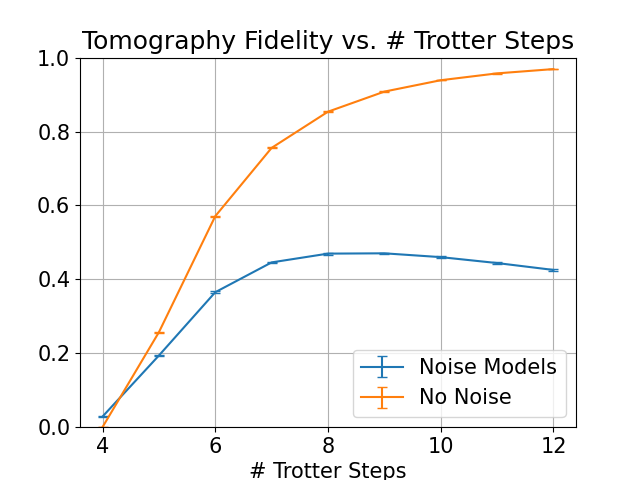
\includegraphics[width=0.5\textwidth]{../TomographyFidelities.png}
\caption{We compare how the number of trotter steps affects fidelity with and without noise. Both results were obtained using a simulator on a classical computer. The orange line shows the fidelity on a perfect quantum computer (no noise), and the blue line uses Qiskit noise models to predict how the fidelity would behave on a real device.}
\label{fig:SimFids}
\end{figure}

\section{Ibmq Jakarta Results}

While we were able to obtain access to \texttt{ibmq\_jakarta} for some jobs, the wait time was too long for it to be practical to recreate figure \ref{fig:SimFids} with results from the real device. Instead, we chose a fixed number of trotter steps (N=7) and computed the quantum fidelity on 6 repetitions. Like before, we performed 8192 measurements in each basis on each repetition. The average fidelity we obtained was $0.24 \pm .01$. While this is less than half the number of repetitions we had in the simulations, the standard deviation is so small that it is highly unlikely additional repetitions would be informative in any meaningful way.

The average fidelity for N=7 trotter steps on the noisy simulator was $0.45 \pm .001$. Given the small uncertainties on both fidelities, we can conclude the real device's performance is substantially worse than the noisy simulator and that this performance difference statistically significant.

\section{Conclusion}

\bibliography{ProjectReportBib}

\end{document}